%%%%%%%%%%%%%%%%%%%%  練習問題（旧 prob_p5.png / prob_p6.png / prob_p7.png）  %%%%%%%%%%%%%%%%%%%%
\Rank{A問題}

\Mon{基本事項の確認}

\hspace{1zw}以下の設問に答えよ．ただし，重力加速度の大きさを$9.8\U{m/s^2}$とせよ．
\begin{komon}
\ko{1} 塔の上から小石を自由落下させたところ，$2.0\U{s}$後に地面に達した．塔の高さは何$\U{m}$か．また，小石が地面に達する直前の速さは何$\U{m/s}$か．
\ko{2} ビルの屋上から，初速度$9.8\U{m/s}$でボールを投げ下ろした．$3.0\U{s}$後の速さは何$\U{m/s}$か．
\ko{3} 初速度$19.6\U{m/s}$で地面から小球を鉛直上向きに投げ上げた．$2.0\U{s}$後の速さは何$\U{m/s}$か，また，そのとき地面からの高さは何$\U{m}$か．
\ko{4} 物体を水平方向に初速度$20\U{m/s}$で投げたとき，$3.0\U{s}$後の水平方向の移動距離と鉛直方向の落下距離はそれぞれ何$\U{m}$か．
\ko{5} ボールを地面から斜め$30^\circ$の方向に，初速度$20\U{m/s}$で投げ出した．$1.0\U{s}$後の速度の水平成分と鉛直成分は何$\U{m/s}$か．
\ko{6} ゴルフボールを水平な地面から斜め$30^\circ$の方向に，初速度$19.6\U{m/s}$で打ち上げた．最高点に達するまでの時間は何$\U{s}$か．
\end{komon}

\Rank{B問題}

\Mon{鉛直投げ下げと自由落下}

\hspace{1zw}ある点から小石$\mathrm{A}$を自由落下させ，$1.0\U{s}$後に同じ高さの点から小石$\mathrm{B}$をある速さで投げ下ろしたところ，$\mathrm{B}$は投げ下ろしてから$2.0\U{s}$後に$\mathrm{A}$に追いついた．重力加速度の大きさを$9.8\U{m/s^2}$として，以下の問いに答えよ．
\begin{komon}
\ko{1} 小石$\mathrm{B}$に追いつかれるまでに小石$\mathrm{A}$はどれだけ落下したかを求めよ．
\ko{2} 小石$\mathrm{B}$の初速度の大きさを求めよ．
\end{komon}

\Mon{鉛直投げ上げ}\Sitei

\begin{zuright}{52mm}
\hspace{1zw}地面から高さ$h\U{m}$のビルの屋上から，小石を初速$v_0\U{m/s}$で真上に投げ上げた．重力加速度の大きさを$g\U{m/s^2}$として，以下の問いに答えよ．
\begin{komon}
\ko{1} 最高点に達するまでの時間と，地面から最高点までの高さを求めよ．
\ko{2} 地面に達するまでの時間と，地面に達する直前の速さを求めよ．
\end{komon}
\zusep
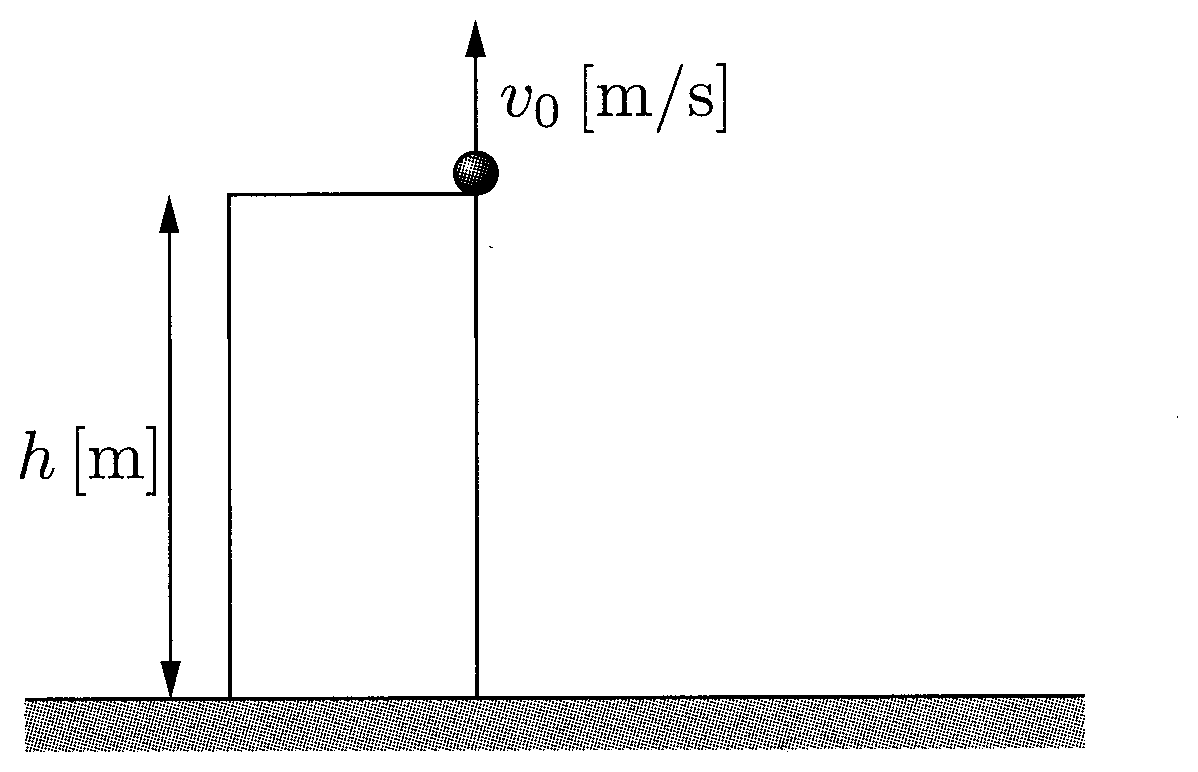
\includegraphics[keepaspectratio,width=52mm]{fig/ch2_p5_up.png}
\end{zuright}

\Mon{水平投射}

\begin{zuright}{48mm}
\hspace{1zw}地面から高さ$h\U{m}$のビルの屋上から，水平右向きに初速$v_0\U{m/s}$で小石を投げた．重力加速度の大きさを$g\U{m/s^2}$として，以下の問いに答えよ．
\begin{komon}
\ko{1} 小石を投げてから地面に達するまでの時間を求めよ．
\ko{2} ビルから小石の落下点までの水平距離を求めよ．
\ko{3} 小石が地面に達する直前の速さを求めよ．
\end{komon}
\zusep
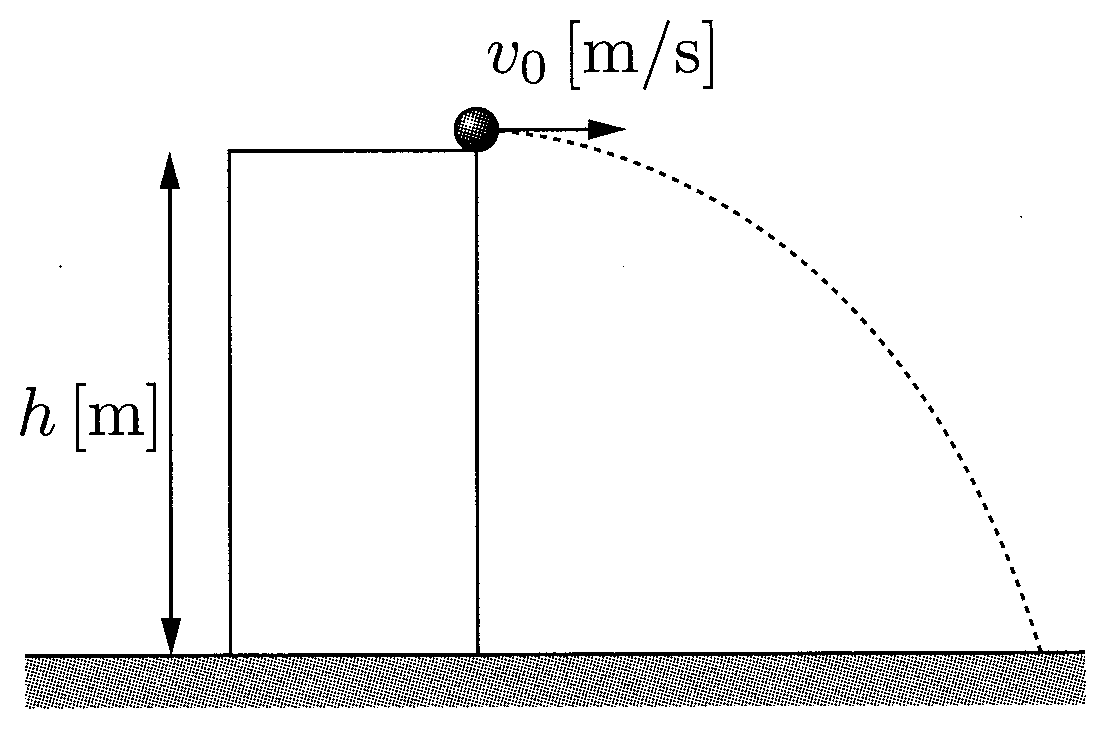
\includegraphics[keepaspectratio,width=48mm]{fig/ch2_p5_hor.png}
\end{zuright}

\Mon{斜方投射}\Sitei

\begin{zuright}{52mm}
\hspace{1zw}地面から仰角$\theta\U{rad}$の向きに初速$v_0\U{m/s}$でボールを投げた．投げた点を原点$\mathrm{O}$とし，図のように水平右向きに$x$軸，鉛直上向きに$y$軸を取る．重力加速度の大きさを$g\U{m/s^2}$として以下の問いに答えよ．
\begin{komon}
\ko{1} 投げてから時間$t\U{s}$後の$x,y$座標を求めよ．
\ko{2} 投げてから最高点に達するまでの時間を求めよ．また，そのときの$y$座標を求めよ．
\ko{3} ボールの水平到達距離を求めよ．
\end{komon}
\zusep
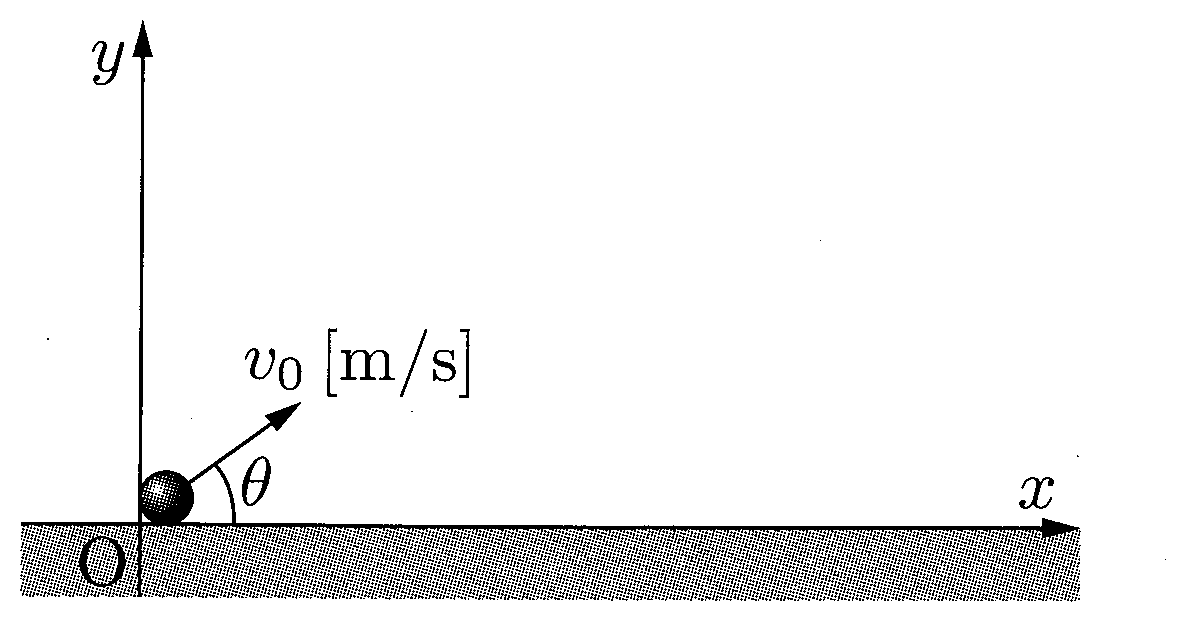
\includegraphics[keepaspectratio,width=52mm]{fig/ch2_p6_obl.png}
\end{zuright}

\Mon{斜方投射}

\begin{zuright}{48mm}
\hspace{1zw}地上から高さ$h\U{m}$のビルの屋上から，初速$v_0\U{m/s}$，仰角$\theta\U{rad}$でボールを投げた．重力加速度の大きさを$g\U{m/s^2}$として，以下の問いに答えよ．
\begin{komon}
\ko{1} 投げてから最高点に達するまでの時間を求めよ．
\ko{2} 投げてからボールが地面に落下するまでに要する時間を求めよ．
\ko{3} 投げた点から落下点までの水平方向の移動距離を求めよ．
\ko{4} 落下点におけるボールの速度の水平成分と鉛直成分を求めよ．
\end{komon}
\zusep
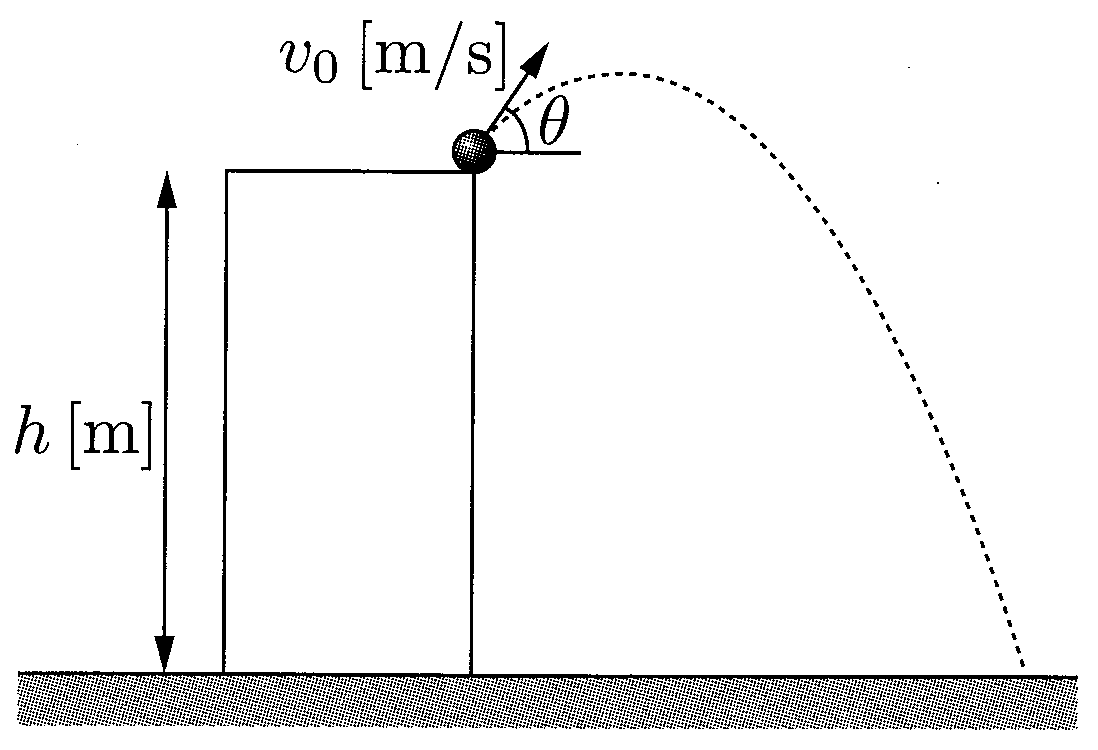
\includegraphics[keepaspectratio,width=48mm]{fig/ch2_p6_bldg.png}
\end{zuright}

\Mon{自由落下と鉛直投げ上げ}

\hspace{1zw}地面から高さ$h\U{m}$のビルの屋上から小石$\mathrm{A}$を自由に落下させた．$\mathrm{A}$を手放すと同時に小石$\mathrm{B}$を地面から初速$v_0\U{m/s}$で鉛直上向きに投げ上げたところ，$\mathrm{A}$と$\mathrm{B}$は衝突した．重力加速度の大きさを$g\U{m/s^2}$として，以下の問いに答えよ．
\begin{komon}
\ko{1} 運動を始めてから$\mathrm{A}$と$\mathrm{B}$が衝突するまでの時間を求めよ．
\ko{2} $\mathrm{A}$と$\mathrm{B}$が衝突する点の，地上からの高さを求めよ．
\end{komon}

\Rank{C問題}

\Mon{鉛直投げ上げと等速度運動}

\hspace{1zw}一定の速さ$7.0\U{m/s}$で下降している気球から，小石を鉛直上向きに投げたら，$3.0\U{s}$後に小石が気球を追い越して落ちていった．さらに$4.0\U{s}$後には小石は地上に達した．重力加速度の大きさを$9.8\U{m/s^2}$として，以下の問いに答えよ．
\begin{komon}
\ko{1} 小石を投げてから小石が気球を追い越すまでに気球が下降した距離を求めよ．
\ko{2} 小石が気球を追い越す瞬間における，小石の地面に対する速さを求めよ．
\ko{3} 小石が地面に達したときの気球の地面からの高さを求めよ．
\end{komon}

\Mon{放物運動}

\begin{zuright}{50mm}
\hspace{1zw}右図のように，一定の速さ$v\U{m/s}$で運動している台車が点$\mathrm{A}$を通過する瞬間に，台車からボールを初速度$u\U{m/s}$で鉛直上向きに打ち出したところ，ボールは点$\mathrm{B}$で台車に落下した．
\zusep
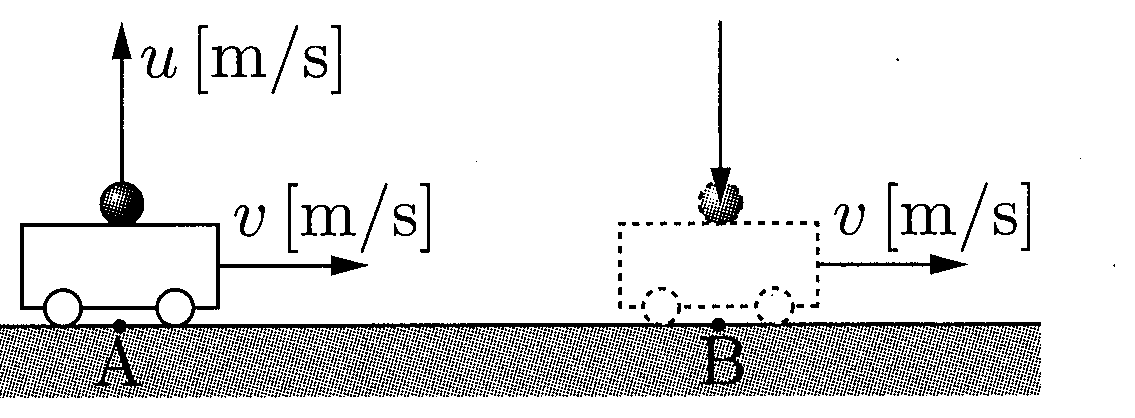
\includegraphics[keepaspectratio,width=50mm]{fig/ch2_p7_cart.png}
\end{zuright}
\vspace{-\medskipamount}
\hspace{1zw}$u\U{m/s}$が台車に対するボールの相対速度であることに注意して，以下の設問に答えよ．重力加速度の大きさを$g\U{m/s^2}$とする．
\begin{komon}
\ko{1} $\mathrm{AB}$間の水平距離を求めよ．
\end{komon}
\hspace{1zw}次に，台車の速さを$\dfrac{1}{2}v\U{m/s}$にして，点$\mathrm{A}$を通過する瞬間に台車からボールをある初速度で鉛直上向きに打ち上げたところ，ボールは先ほどと全く同じ点$\mathrm{B}$で台車に落下した．
\begin{komon}
\ko{2} ボールの鉛直方向の初速度は先ほどの場合の何倍か．
\ko{3} ボールが到達した最高点の高さは先ほどの場合の何倍か．
\end{komon}

\Mon{モンキーハンティング}

\begin{zuright}{47mm}
\hspace{1zw}右図のように水平な地上で，点$\mathrm{O}$から水平距離$l\U{m}$だけ離れた点$\mathrm{B}$の真上の高さ$h\U{m}$の点$\mathrm{A}$から物体$\mathrm{P}$を自由落下させると同時に，点$\mathrm{O}$から物体$\mathrm{Q}$を仰角$\theta\U{rad}$，初速$v_0\U{m/s}$で投げ出した．投げ出した時刻を$0\U{s}$とし，右図のように$x,y$軸をとる．重力加速度の大きさを$g\U{m/s^2}$として以下の問いに答えよ．
\begin{komon}
\ko{1} 時刻$t\U{s}$における$\mathrm{P}$から$\mathrm{Q}$までの距離を求めよ．
\ko{2} 時刻$t\U{s}$における$\mathrm{P}$から見た$\mathrm{Q}$の相対速度の水平成分および鉛直成分を求めよ．
\end{komon}
\zusep
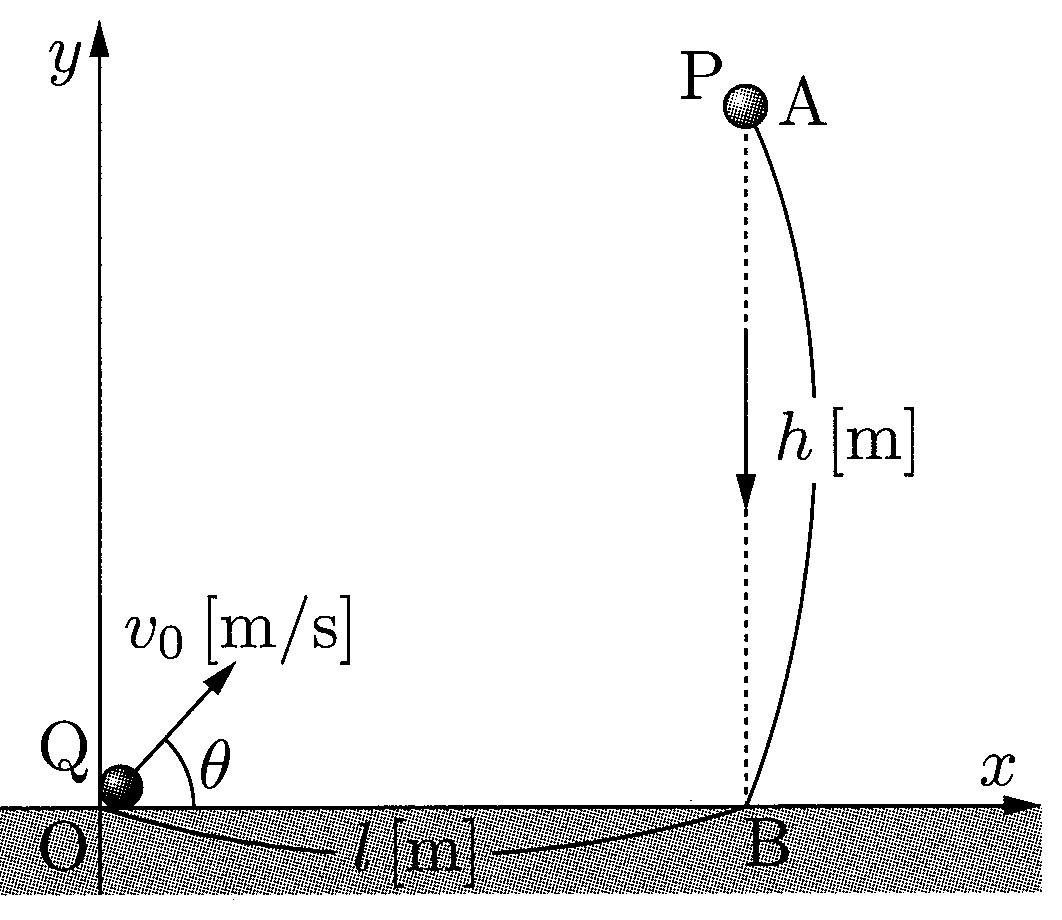
\includegraphics[keepaspectratio,width=47mm]{fig/ch2_p7_monkey.png}
\end{zuright}
\begin{komon}
\ko{3} $\mathrm{Q}$が$\mathrm{P}$に命中するためには，$\theta,l,h$の間にはどのような条件式が成立していなければならないか．
\ko{4} 地上に落下するまでに$\mathrm{Q}$が$\mathrm{P}$に命中するには，初速$v_0$にどのような条件が必要か．$g,l,\theta$を用いて表せ．
\end{komon}
